\chapter{Calculator With Friendly Output}
\label{chapter:calc}
\graphicspath{{./Lab06Calculator/Fig}}

\section{Outcomes and Objectives}

The outcome of this lab is to instantiate a calculator with signed
decimal output making it easy for anyone to use the circuit.
Through this process you will achieve the following
learning objectives.
\begin{itemize}
	\item \Paste{bok:REP_WordStatement}
	\item \Paste{bok:REP_TruthTable}
\end{itemize}



\section{Basic Calculator}

This week you are going to build a very basic calculator that can add or
subtract 4-bit values using the input and output shown in 
Figure~\ref{fig:calcDevBoard}.

\begin{figure}[ht]
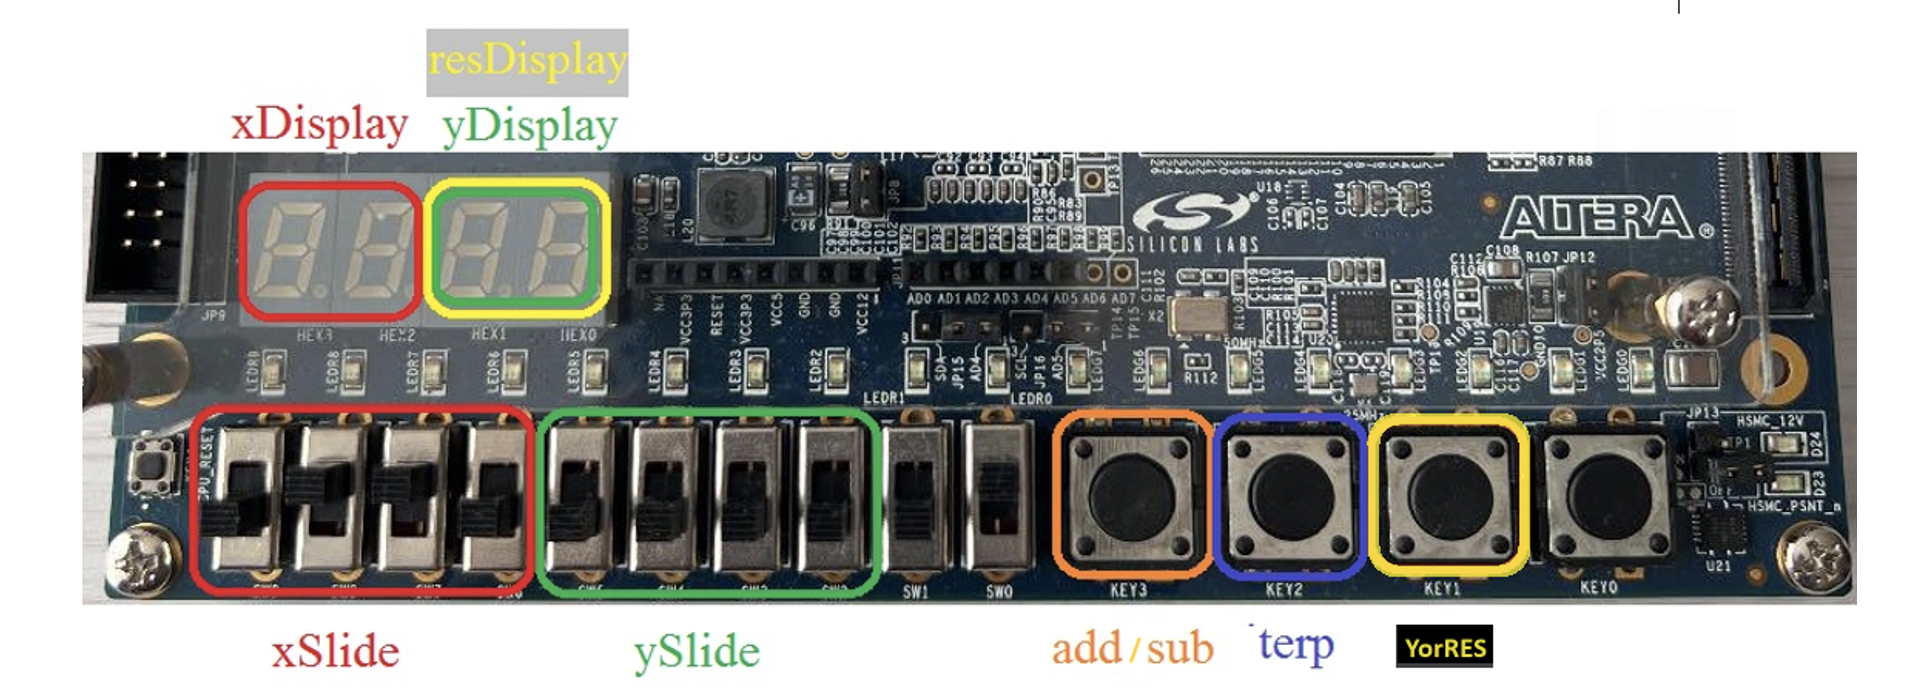
\includegraphics{ image1.png}
\caption{The input and output of the calculator digital circuit.}
\label{fig:calcDevBoard}
\end{figure}

On the surface, this should require nothing more
than connecting some slide switches to the x and y inputs of an
adder/subtractor which sends its output to a 7-segment display. And for
the most part this is correct. However, instead of displaying the input
and output of the adder as hexadecimal values, you will display them as
2-digit decimal values. 

The user input and output are shown in Figure~\ref{fig:calcDevBoard}.
The user enters a pair of 4-bit operands using the left-most slide
switches, \textbf{xSlide} and \textbf{ySlide}. The value entered for
\textbf{xSlide} is displayed on the two (red) \textbf{xDisplay}
7-segment displays. The value entered for \textbf{ySlide} is displayed
on the two (green) \textbf{yDisplay} 7-segment displays. The leftmost
the \textbf{addSub} buttons specify the operation performed on
\textbf{xSlide} and \textbf{ySlide}. The result is \textbf{xSlide} +
\textbf{ySlide} or \textbf{xSlide} - \textbf{ySlide}. 



The \textbf{interp} button determines how the values are displayed on the
7-segment display. When unpressed, the 7-segment displays show the
decimal value, when pressed, the 7-segment displays show 2's complement.
This will be explained in the next section. As we have only 4 7SDs on
board, the same 7SD of operand Y will be used to show the operation
result (yellow) when the \textbf{yOrResult} button is pressed.

\section{System Architecture}

The system architecture shown in Figure~\ref{fig:sysArchCalc} shows the adder subtractor
processing the xSlide and ySlide inputs. The 4-bit x, y and result
values are processed by the sigUnsig box before being displayed on the
7-segment displays. It is now time to turn our attention to this module.

\begin{figure}[ht]
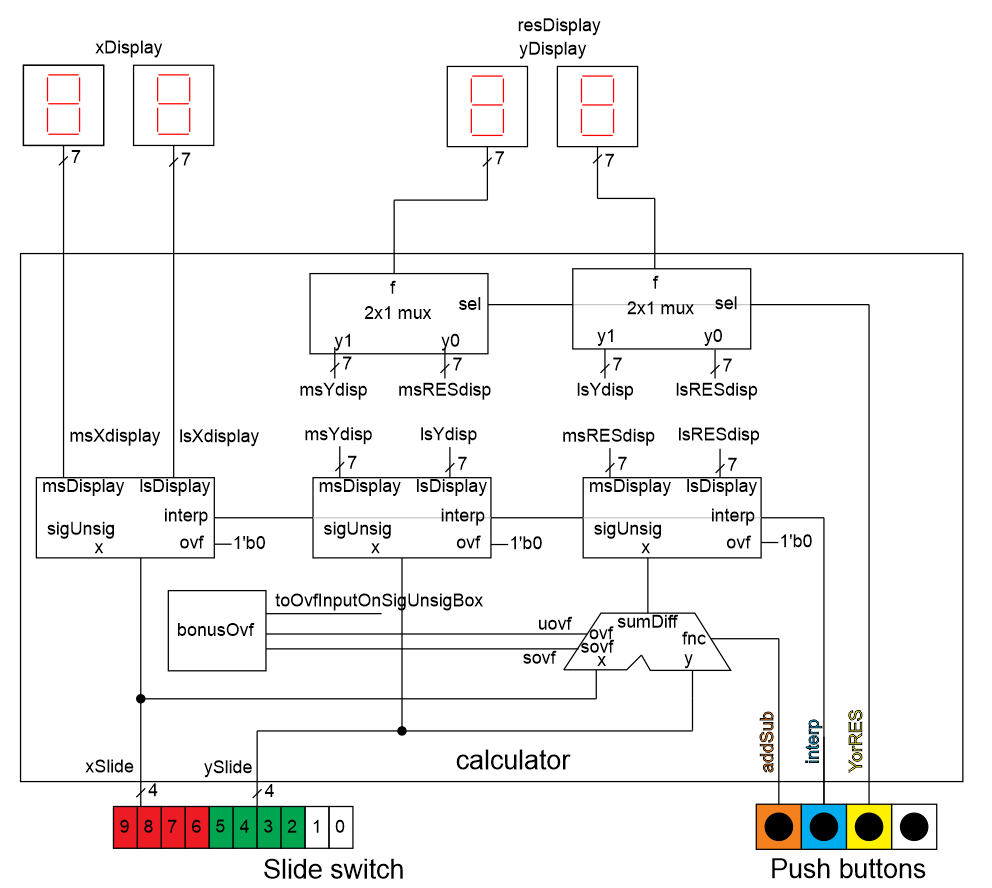
\includegraphics{ image2.png}
\caption{The system architecture of the calculator.}
\label{fig:sysArchCalc}
\end{figure}


\section{Module: sigUnsign}

The significant design problem in today's lab comes in this section,
building the sigUnsig module. This module takes in a 4-bit value and
displays a 2-digit signed or unsigned representation on a pair of
7-segment displays. Before we go into the internal organization of this
module, look at its module declaration in Listing~\ref{listing:cacSigUnsigModule}.


\begin{lstlisting}[language=Verilog,
 caption={Module declaration for the sigUnsig module.},
 label={listing:cacSigUnsigModule},
 frame=single]
 module sigUnsig(x, interp, ovf, msDisplay, lsDisplay);    
    input  wire [3:0]  x;	 	 
    input  wire        interp;
    input  wire        ovf;
    output wire [6:0]  msDisplay, lsDisplay;
 \end{lstlisting}

The 4-bit input \hdl{x} is interpreted as either signed (2's complement
value) when \hdl{interp = 1} or unsigned (regular binary number) when
\hdl{interp = 0}.  The \device{msDisplay} is the most significant (ms)
symbol being displayed and \device{lsDisplay} is the least significant (ls)
symbol being display.  The term ``symbol'' is used because more than
one type of information can be displayed depending on the values
of the inputs.  Let's explore this.

For example, let \hdl{x = 4'b1100}. 
\begin{itemize}
\item 
If \hdl{interp = 1'b0} then
\hdl{x} is interpreted as unsigned and its value is 12. Then
the \device{msDisplay} should show ``1'' and \device{lsDisplay} ``2''. 

\item 
If \hdl{interp = 1'b1} then
\hdl{x} is interpreted as 2's complement and its value is -4. Then
the \device{msDisplay} should show ``-'' and \device{lsDisplay} ``4''. 

\item 
In the previous two cases we assumed, without stating it, that \hdl{ovf = 1'b0}.
If \hdl{ovf = 1'b1} then the operation which generated \hdl{x} overflowed
and the value of \hdl{x} is invalid.  In this case both display's should show ``X''.
Since we are working with 7-segments, our ``X'' looks much more like ``H'' :(
\end{itemize}

Not complete Table~\ref{table:calcSigUnsign} by filling in the values of \hdl{msDisplay} and
\hdl{lsDisplay} for a signed and unsigned interpretation, assuming
\emph{ovf}=0. If the interpreted value is
positive and a single digit then assign \emph{msDisplay} blank. If the
interpreted value is negative then assign \emph{msDisplay} ``-``. If the
interpreted value is greater than 10, assign \emph{msDisplay} ``1''.


\begin{longtable}[]{@{}
|  >{\raggedright\arraybackslash}p{(\columnwidth - 8\tabcolsep) * \real{0.1999}}|
  >{\raggedright\arraybackslash}p{(\columnwidth - 8\tabcolsep) * \real{0.2000}}|
  >{\raggedright\arraybackslash}p{(\columnwidth - 8\tabcolsep) * \real{0.2000}}|
  >{\raggedright\arraybackslash}p{(\columnwidth - 8\tabcolsep) * \real{0.2000}}|
  >{\raggedright\arraybackslash}p{(\columnwidth - 8\tabcolsep) * \real{0.2000}}|@{}}
\caption{The output of the \hdl{sigUnsig} module when \hdl{ovf=0}.}\label{table:calcSigUnsign}\tabularnewline
\toprule()
\multirow{2}{*}{4-bit input x} &
\multicolumn{2}{>{\raggedright\arraybackslash}p{(\columnwidth - 8\tabcolsep) * \real{0.4000} + 2\tabcolsep}}{%
\hdl{interp = 0} Unsigned } 
 &
\multicolumn{2}{>{\raggedright\arraybackslash}p{(\columnwidth - 8\tabcolsep) * \real{0.4000} + 2\tabcolsep}@{}}{%
\hdl{interp = 1} Signed } \\

&\hdl{msDisplay} & \hdl{lsDisplay} & \hdl{msDisplay} & \hdl{lsDisplay} \\

\midrule()
\endfirsthead
\toprule()
\multirow{2}{*}{4-bit input x} &
\multicolumn{2}{>{\raggedright\arraybackslash}p{(\columnwidth - 8\tabcolsep) * \real{0.4000} + 2\tabcolsep}}{%
\emph{interp = 0} Unsigned } 
 &
\multicolumn{2}{>{\raggedright\arraybackslash}p{(\columnwidth - 8\tabcolsep) * \real{0.4000} + 2\tabcolsep}@{}}{%
\emph{interp = 1} Signed } \\

&\hdl{msDisplay} & \hdl{lsDisplay} & \hdl{msDisplay} & \hdl{lsDisplay} \\
\midrule()
\endhead
4'b0000 & blank & 0 & blank & 0 \\ \hline
4'b0001 & & & & \\ \hline
4'b0010 & & & & \\ \hline
4'b0011 & & & & \\ \hline
4'b0100 & & & & \\ \hline
4'b0101 & & & & \\ \hline
4'b0110 & & & & \\ \hline
4'b0111 & & & & \\ \hline
4'b1000 & & & & \\ \hline
4'b1001 & & & & \\ \hline
4'b1010 & & & & \\ \hline
4'b1011 & & & & \\ \hline
4'b1100 & 1 & 2 & - & 4 \\ \hline
4'b1101 & & & & \\ \hline
4'b1110 & & & & \\ \hline
4'b1111 & & & & \\
\bottomrule()
\end{longtable}


Let's look at the patterns in Table~\ref{table:calcSigUnsign}.  These will be helpful when you are
required to fill in the
missing pieces of the architecture of the signUnsign module in Figure~\ref{fig:calcSigUnSigArch}.
\begin{itemize}

	\item \hdl{msDisplay} is assigned one of four values
	\begin{itemize}
		\item  blank when the interpretation of \hdl{x} is an unsigned or signed value less than  10
		\item 1 when the interpretation of \hdl{x} is an unsigned value greater than 10
		\item - when the interpretation of \hdl{x} is signed value less than 0
		\item X when the \hdl{ovf = 1}
	\end{itemize}

	\item \hdl{lsDisplay} is assigned one of four values, 
	\begin{itemize}
		\item \hdl{x} when the interpertation of \hdl{x} is a unsigned or signed value less than 10
		\item \hdl{x-10} when the interpertation of \hdl{x} is an unsigned value greater than 10
		\item \hdl{0-x} when the interpretation of \hdl{x} is a signed value less than 0
		\item X when the \hdl{ovf = 1}
	\end{itemize}
\end{itemize}

\begin{figure}[ht]
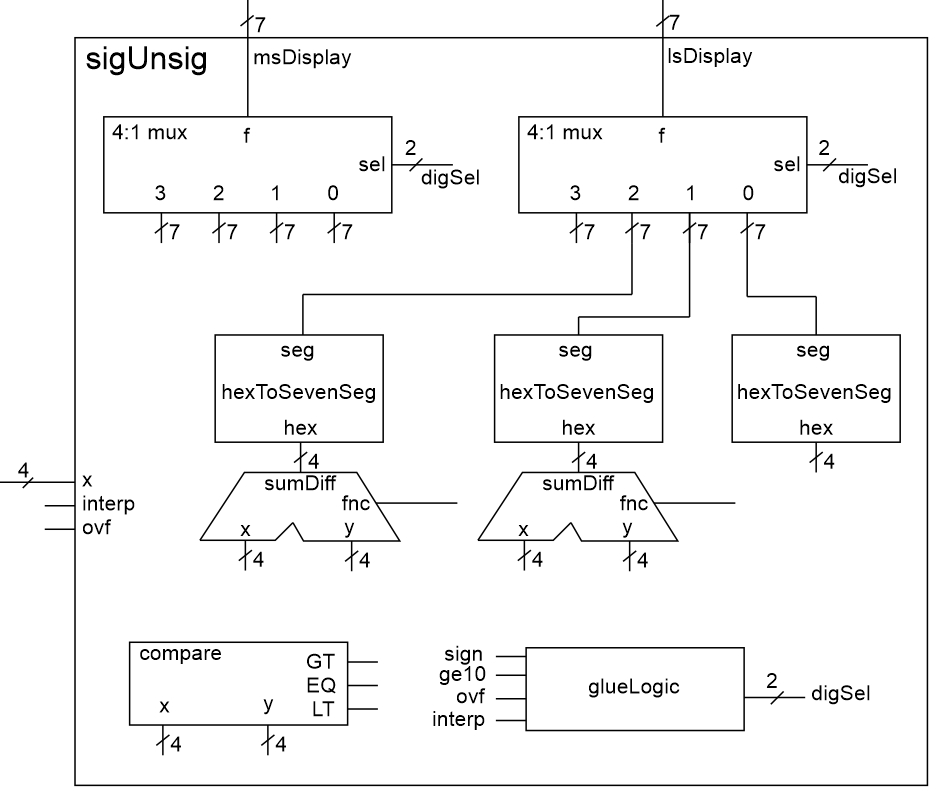
\includegraphics{ image6.png}
\caption{The internal architecture of the signUnsig module.}
\label{fig:calcSigUnSigArch}
\end{figure}



To understand this better, complete Listing~\ref{listing:calcDisplayLogic}. 
You will form the 2's complement of x, the negative of x, by subtracting x
from 0.  You can assign the value blank, -, constants, x, or a function of x 
(e.g. \hdl{x-10}) as needed. Note that this code is NOT to be used in your 
actual code for this lab.


\begin{lstlisting}[language=Verilog,
 caption={Logic that determines the output of the 4:1 muxes in Figure~\ref{fig:calcSevenSeg}.},
 label={listing:calcDisplayLogic},
 frame=single]
if        ( (interp == 0) && (x < 10) ) {			// y0 input
    msDisplay = 		lsDisplay = 	

} else if ( (interp == 0) && (x >= 10) ) {		// y1 input
    msDisplay =		lsDisplay =

} else if ( (interp == 1) && (x >= 0) ) {		// y0 input
    msDisplay =		lsDisplay = 

} else if ( (interp == 1) && (x < 0) ) {			// y2 input
    msDisplay = 		lsDisplay = 

}
\end{lstlisting}



Now that you know what should be displayed on  \device{msDisplay} 
and \device{lsDisplay}, let's look at how we an form these symbols on the
7-segment displays.  In order to do this, you need Figure~\ref{fig:calcSevenSeg},
the bit-order of the segments controlling the illumination o the segments. Remember
that the segments are active low, meaning a logic 0 illuminates a
segment. Thus, the 7-bit code 7'b0100100 illuminates the pattern ``2''.

\begin{figure}[ht]
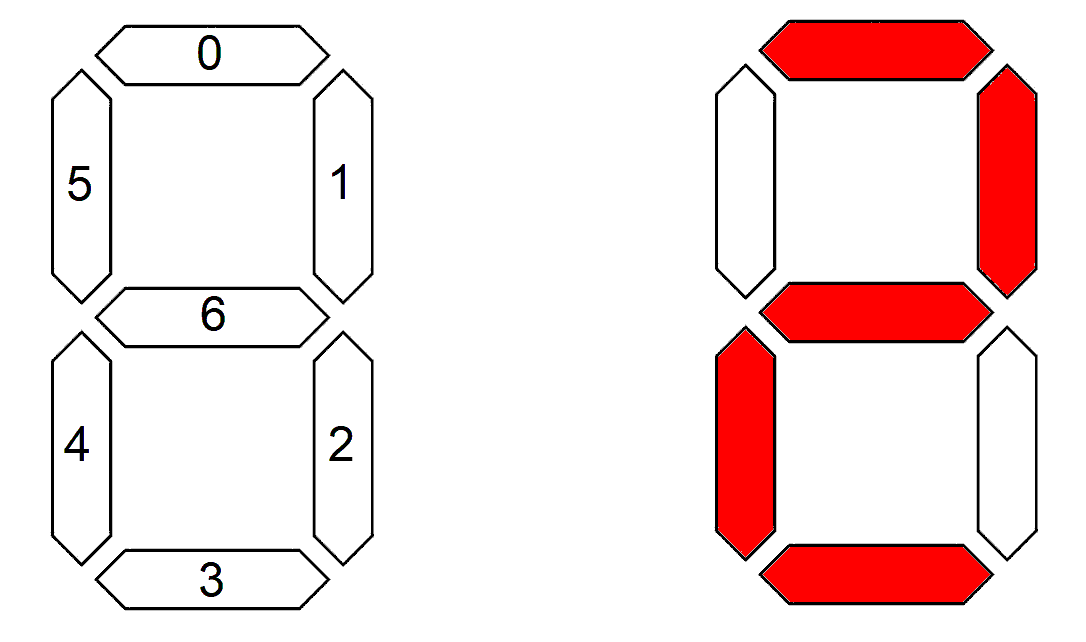
\includegraphics[width=0.3\paperwidth]{ image3.png}
\caption{The logical arrangements of the segments in a 7-segment display.}
\label{fig:calcSevenSeg}
\end{figure}

Test your understanding o the \hdl{signUnsign} output by completing
Table~\ref{table:calcSevenSeg}. Do this by coloring in the segments of the 
7-segment displays that are illuminated for each of the inputs. Then write 
the binary and hexadecimal value to illuminate those patterns to the 
right of \hdl{msDisplay=7'b} and \hdl{lsDisplay=7'b}.

\begin{longtable}[]{@{}
|  >{\raggedright\arraybackslash}p{(\columnwidth - 8\tabcolsep) * \real{0.1458}}|
  >{\raggedright\arraybackslash}p{(\columnwidth - 8\tabcolsep) * \real{0.3170}}|
  >{\raggedright\arraybackslash}p{(\columnwidth - 8\tabcolsep) * \real{0.02}}|
  >{\raggedright\arraybackslash}p{(\columnwidth - 8\tabcolsep) * \real{0.1458}}|
  >{\raggedright\arraybackslash}p{(\columnwidth - 8\tabcolsep) * \real{0.3170}}|@{}}
\caption{For each set of inputs to the signUnsig module, determine the 7-segment display pattern.}\label{table:calcSevenSeg} \tabularnewline
\toprule()
Input & 7-segment pattern & & Input & 7-segment pattern \\
\midrule()
\endfirsthead
\toprule()
Input & 7-segment pattern & & Input & 7-segment pattern \\
\midrule()
\endhead
4'b0010

interp = 1

ovf = 0 &

\vspace{0.1cm}
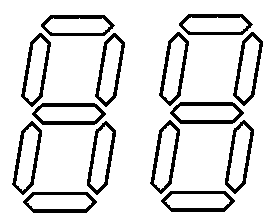
\includegraphics{ image4.png}
\vspace{0.1cm}

msDisplay = 7'b

lsDisplay = 7'b & & 4'b0111

interp = 0

ovf = 0 &

\vspace{0.1cm}
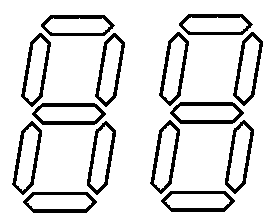
\includegraphics{ image4.png}
\vspace{0.1cm}

msDisplay = 7'b

lsDisplay =7'b \\ \hline
4'b1100

interp = 0

ovf = 0 &

\vspace{0.1cm}
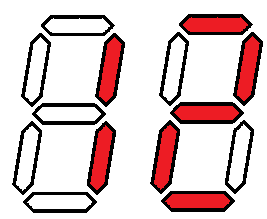
\includegraphics{ image5.png}
\vspace{0.1cm}

msDisplay = 7'b1111001 = 7'h79

lsDisplay =7'b0100100 = 7'h24 & & 4'b1000

interp = 1

ovf = 0 &

\vspace{0.1cm}
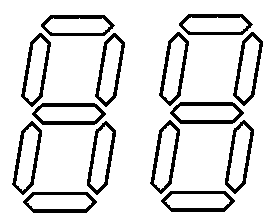
\includegraphics{ image4.png}
\vspace{0.1cm}

msDisplay = 7'b

lsDisplay =7'b \\ \hline
4'b1100

interp = 1

ovf = 0 &

\vspace{0.1cm}
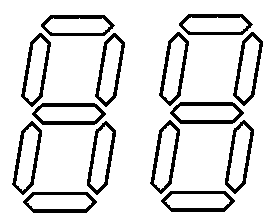
\includegraphics{ image4.png}
\vspace{0.1cm}

msDisplay = 7'b

lsDisplay =7'b & & 4'b1010

interp = 1

ovf = 1 &

\vspace{0.1cm}
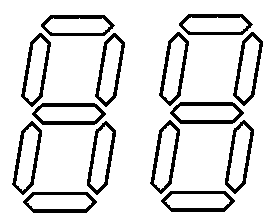
\includegraphics{ image4.png}
\vspace{0.1cm}

msDisplay = 7'b

lsDisplay = 7'b \\ \hline
\bottomrule()
\end{longtable}

Now we are ready to put the pieces of the sigUnsig module together. The
building blocks in Figure~\ref{fig:calcSigUnSigArch} are captured in the organization described
by Listing~\ref{listing:calcDisplayLogic}, along with some extra hardware.


You are responsible for connecting the inputs of the 4:1 mux and adder
subtractors using the logic described in Listing~\ref{listing:calcDisplayLogic}. To help you do this,
first complete Table~\ref{table:calcMuxLogic}. Take notice of the comments in the Listing~\ref{listing:calcDisplayLogic} to
determine which data inputs to associate with each of the muxes 4 data
inputs. You should associate the overflow case with the y3 input.

\begin{longtable}[]{@{}
| >{\raggedright\arraybackslash}p{(\columnwidth - 8\tabcolsep) * \real{0.1999}}|
  >{\raggedright\arraybackslash}p{(\columnwidth - 8\tabcolsep) * \real{0.2000}}|
  >{\raggedright\arraybackslash}p{(\columnwidth - 8\tabcolsep) * \real{0.2000}}|
  >{\raggedright\arraybackslash}p{(\columnwidth - 8\tabcolsep) * \real{0.2000}}|
  >{\raggedright\arraybackslash}p{(\columnwidth - 8\tabcolsep) * \real{0.2000}}|@{}}
\caption{The input values to the 4:1 muxes in Figure~\ref{fig:calcSigUnSigArch}.}\label{table:calcMuxLogic}\tabularnewline
\toprule()
\begin{minipage}[b]{\linewidth}\raggedright
input
\end{minipage} & \begin{minipage}[b]{\linewidth}\raggedright
y3
\end{minipage} & \begin{minipage}[b]{\linewidth}\raggedright
y2
\end{minipage} & \begin{minipage}[b]{\linewidth}\raggedright
y1
\end{minipage} & \begin{minipage}[b]{\linewidth}\raggedright
y0
\end{minipage} \\
\midrule()
\endfirsthead
\toprule()
\begin{minipage}[b]{\linewidth}\raggedright
input
\end{minipage} & \begin{minipage}[b]{\linewidth}\raggedright
y3
\end{minipage} & \begin{minipage}[b]{\linewidth}\raggedright
y2
\end{minipage} & \begin{minipage}[b]{\linewidth}\raggedright
y1
\end{minipage} & \begin{minipage}[b]{\linewidth}\raggedright
y0
\end{minipage} \\
\midrule()
\endhead
digSel & 2'b11 & & & \\ \hline
msDisplay & ``X'' & & 1 & \\ \hline
lsDisplay & & & & x \\
\bottomrule()
\end{longtable}

In addition, you should add the following to Figure~\ref{fig:calcSigUnSigArch}:

\begin{itemize}
\item
  Wire the inputs of the comparator to determine to generate a signal
  xGE10 which is logic 1 when x is greater than or equal to 10.
\item
  Wire the inputs of the adder subtractor according to Table~\ref{table:calcMuxLogic}.
\item
  Wire the input of the rightmost hexToSevenSeg .
\end{itemize}

The last step in building this module is to describe the behavior of the
glueLogic box. This function chooses which input of the 4 mux inputs to
route to the output. Before you do this, you will need to create a
signal \emph{sign} which equals 1 when x represents a negative value
(when interpreted as a signed value) and equals to 0 when x represents a
positive value (when interpreted as a signed value). Logically speaking,
this is a trivial operation -- it does not require any logic gates.

Now, we can examine the contents of the glueLogic box. Do this by
completing the truth table in Table~\ref{table:calcGlueLogic}.

\begin{longtable}[]{@{}
|  >{\raggedright\arraybackslash}p{(\columnwidth - 8\tabcolsep) * \real{0.1999}}|
  >{\raggedright\arraybackslash}p{(\columnwidth - 8\tabcolsep) * \real{0.2000}}|
  >{\raggedright\arraybackslash}p{(\columnwidth - 8\tabcolsep) * \real{0.2000}}|
  >{\raggedright\arraybackslash}p{(\columnwidth - 8\tabcolsep) * \real{0.2000}}|
  >{\raggedright\arraybackslash}p{(\columnwidth - 8\tabcolsep) * \real{0.2000}}|@{}}
\caption{Truth table for the glueLogic box.}\label{table:calcGlueLogic}\tabularnewline
\toprule()
\begin{minipage}[b]{\linewidth}\raggedright
ovf
\end{minipage} & \begin{minipage}[b]{\linewidth}\raggedright
interp
\end{minipage} & \begin{minipage}[b]{\linewidth}\raggedright
sign
\end{minipage} & \begin{minipage}[b]{\linewidth}\raggedright
xGE10
\end{minipage} & \begin{minipage}[b]{\linewidth}\raggedright
digSel
\end{minipage} \\
\midrule()
\endfirsthead
\toprule()
\begin{minipage}[b]{\linewidth}\raggedright
ovf
\end{minipage} & \begin{minipage}[b]{\linewidth}\raggedright
interp
\end{minipage} & \begin{minipage}[b]{\linewidth}\raggedright
sign
\end{minipage} & \begin{minipage}[b]{\linewidth}\raggedright
xGE10
\end{minipage} & \begin{minipage}[b]{\linewidth}\raggedright
digSel
\end{minipage} \\
\midrule()
\endhead
1 & x & x & x & \\ \hline
0 & 0 & x & 0 & \\ \hline
0 & 0 & x & 1 & \\ \hline
0 & 1 & 0 & x & \\ \hline
0 & 1 & 1 & x & \\
\bottomrule()
\end{longtable}


It would make sense to use an always case statement to realize the logic
in Listing~\ref{listing:calcDisplayLogic}. However, an always case statement requires each of the 16
difference cases to be explicitly enumerated. However, the truth table
in Listing~\ref{listing:calcDisplayLogic} is most efficiently described using don't cares in the
input. Fortunately, the always/casez variation (note the ``z'' at the
end of ``case'') allows don't cares in the input in the form of ``?''.
For example, for the second row in Listing~\ref{listing:calcDisplayLogic}, the \{ovf, interp, sign,
xGE10\} vector has don't cares for the \emph{sign} value. Therefore, the
case for this row is 4'b01?0. \uline{It is imperative that you include a
``default'' case whenever you use a always/case statement.} This
combination of cases is shown in Listing~\ref{listing:cacAlwaysStaement}.


\begin{lstlisting}[language=Verilog,
 caption={The always/casez statement allows don't cares in the input.},
 label={listing:cacAlwaysStaement},
 frame=single]
 always @(*)
    casez ({ovf, interp, xGE10, x[3]})
        4'b01?0: digSel = 2'b00;
        default: digSel = 2'b11;
    endcase

 \end{lstlisting}


\protect\hypertarget{sigUnsign_Verilog}{}{}The Verilog code for the
signUnsig module consists of 8 instantiation statements and an
always/casez statement. For this module, I want you to:

\begin{itemize}
\item
  Use the module declaration given in Listing~\ref{listing:cacSigUnsigModule}.
\item
  Use the module definitions for

  \begin{itemize}
  \item
    Generic Mux4x1 posted on this lab's Canvas folder
  \item
    sevenSegment created in lab 02
  \item
    genericAdderSubtractor posted on a previous lab's Canvas folder
  \item
    genericComparator posted on a previous lab's Canvas folder
  \end{itemize}
\item
  Use localparm to give names to the 7-bit constant patterns (fill in
  the values for x).

  \begin{itemize}
  \item
    localparam {[}6:0{]} displayBlank = 7'bxxxxxxx;
  \item
    localparam {[}6:0{]} displayOne = 7'bxxxxxxx;
  \item
    localparam {[}6:0{]} displayMinus = 7'bxxxxxxx;
  \item
    localparam {[}6:0{]} displayX = 7'bxxxxxxx;
  \end{itemize}
\item
  Provide meaningful names to the wires in the module.
\item
  Properly tab-indent your code

  \begin{itemize}
  \item
    Single level for wire declarations
  \item
    Single level for component instantiations
  \item
    Two levels for casez statement
  \item
    Three levels for casez values
  \end{itemize}
\end{itemize}

\section{Bonus: Ovf Logic}

The default configuration of the system architecture ignores any
overflow generated by the adder subtractor. If you choose, you may
implement the logic necessary to determine if overflow occurs in the
selected interpretation. In order to receive credit, your circuit needs
to work under \uline{all combination} of addSub and interp. Overflow for
unsigned subtraction will require some careful analysis.

Your solution should have 2 LEDs, one for signed and one for unsigned.
The unsigned overflow LED should illuminate when overflow will occur if
the numbers are interpreted as unsigned numbers. The signed overflow LED
is on when an overflow will occur if the numbers are interpreted as
two's complement numbers.

For example, if the x and y inputs are 1001 and the operation is
addition, then both signed and unsigned LEDs will illuminate.


\section{Pin-Assignment}

Use the image of the development board in Figure~\ref{fig:calcDevBoard} in and the
information in the Cyclone V GX Kit User Manual (posted on the class web
page) to determine the FPGA pins associated with the input and output
devices used by the calculator module

\begin{longtable}[]{@{}
|  >{\raggedright\arraybackslash}p{(\columnwidth - 8\tabcolsep) * \real{0.1436}}|
  >{\raggedright\arraybackslash}p{(\columnwidth - 8\tabcolsep) * \real{0.1829}}|
  >{\raggedright\arraybackslash}p{(\columnwidth - 8\tabcolsep) * \real{0.1665}}|
  >{\raggedright\arraybackslash}p{(\columnwidth - 8\tabcolsep) * \real{0.2621}}|
  >{\raggedright\arraybackslash}p{(\columnwidth - 8\tabcolsep) * \real{0.2448}}|@{}}
  \caption{Pin Assignment for the calculator.}\label{table:calcPinAssignment}\tabularnewline
\toprule()
\begin{minipage}[b]{\linewidth}\raggedright
Segment
\end{minipage} & \begin{minipage}[b]{\linewidth}\raggedright
msXdisplay
\end{minipage} & \begin{minipage}[b]{\linewidth}\raggedright
lsXdisplay
\end{minipage} & \begin{minipage}[b]{\linewidth}\raggedright
msYorRESdisplay
\end{minipage} & \begin{minipage}[b]{\linewidth}\raggedright
lsYorRESdisplay
\end{minipage} \\
\midrule()
\endhead
seg{[}6{]} &AC22 & & & \\ \hline
seg{[}5{]} & & W21 & & \\ \hline
seg{[}4{]} & & & AE25& \\ \hline
seg{[}3{]} & & & & W18\\ \hline
seg{[}2{]} & & & & \\ \hline
seg{[}1{]} & & & & \\ \hline
seg{[}0{]} & & & & \\
\bottomrule()
\end{longtable}

\begin{longtable}[]{@{}
|  >{\raggedright\arraybackslash}p{(\columnwidth - 4\tabcolsep) * \real{0.3397}}|
  >{\raggedright\arraybackslash}p{(\columnwidth - 4\tabcolsep) * \real{0.3278}}|
  >{\raggedright\arraybackslash}p{(\columnwidth - 4\tabcolsep) * \real{0.3325}}|@{}}
\toprule()
\begin{minipage}[b]{\linewidth}\raggedright
\end{minipage} & \begin{minipage}[b]{\linewidth}\raggedright
x
\end{minipage} & \begin{minipage}[b]{\linewidth}\raggedright
y
\end{minipage} \\
\midrule()
\endhead
slide{[}3{]} & AE19& \\ \hline
slide{[}2{]} & & W11\\ \hline
slide{[}1{]} & & \\ \hline
slide{[}0{]} & & \\
\bottomrule()
\end{longtable}

\begin{longtable}[]{@{}
|  >{\raggedright\arraybackslash}p{(\columnwidth - 4\tabcolsep) * \real{0.3334}}|
  >{\raggedright\arraybackslash}p{(\columnwidth - 4\tabcolsep) * \real{0.3334}}|
  >{\raggedright\arraybackslash}p{(\columnwidth - 4\tabcolsep) * \real{0.3333}}|@{}}
\toprule()
YorRES & Key{[}1{]} & P12 \\
\midrule()
\endhead
interp & Key{[}2{]} & \\ \hline
addSub & Key{[}3{]} & \\ \hline
\bottomrule()
\end{longtable}

\section{Turn in}

You may work in teams of at most two. Make a record of your response to
the items below and turn them in a single copy as your team's solution
on Canvas using the instructions posted there. Include the names of both
team members at the top of your solutions. Use complete English
sentences to introduce what each of the following listed items (below)
is and how it was derived. In addition to this submission, you will be
expected to demonstrate your circuit at the beginning of your lab
section next week.

\subsubsection{signUnsig Module}

\begin{itemize}
\item
  Complete Table~\ref{table:calcSevenSeg}.
\item
  Complete Table~\ref{table:calcSigUnsign}.
\item
  Complete the code in Listing~\ref{listing:calcDisplayLogic}.
\item
  Complete Figure~\ref{fig:calcSigUnSigArch}, including:

  \begin{itemize}
  \item
    Constant values on inputs of 4:1 mux
  \item
    Constant value on the input of the right-most hexToSeventSeg
  \item
    Value on the input of the adder subtractors
  \item
    Values on the input of the comparator
  \end{itemize}
\item
  Complete Table~\ref{table:calcMuxLogic}.
\item
  Complete Table~\ref{table:calcGlueLogic}.
\item
  \protect\hyperlink{sigUnsign_Verilog}{Verilog code for the body of the
  sigUnsig module} (courier 8-point font single spaced), leave out
  header comments.
\item
  Run the testbench for the sigUnsig module provided on Canvas. Produce
  a timing diagram with the following characteristics. Zoom to fill the
  available horizontal space with the waveform. Color inputs green and
  outputs red. Order the traces from top to bottom as

  \begin{tabular}{p{3cm}p{3cm}p{3cm}}
  signal			& radix				& Color for trace \\ \hline
    x radix 		&	unsigned 		& Green  \\
    xMinus10 		&	 unsigned 	& Green  \\
    x 				&  decimal 		& Cyan  \\
    negativeX 		&  decimal 		& Cyan  \\
    interp 			& default 			& Green  \\
    ovf 			& default 			& Green  \\
    digSel 			&  unsigned 		& Yellow  \\
    xGE10 		& default 			& Yellow  \\
    msDisplay 		&  hex 			& Red  \\
    lsDisplay 		&  hex 			& Red  \\
  \end{tabular}
\end{itemize}

I do not want the signals from the testbench, but rather the signals
from inside the sigUnsig module. You can do this in sigUnsig, by
expanding the sigUnsig\_tb instance in the left ModelSim pane and
selecting ``uut''. Since uut is an instance of the sigUnsig module, all
the signals accessible in the sigUnsig module are shown in the center
Object. You can add duplicates of signals by repeating the drag-and-drop
operation.

Your completed timing diagram should look something like the following.

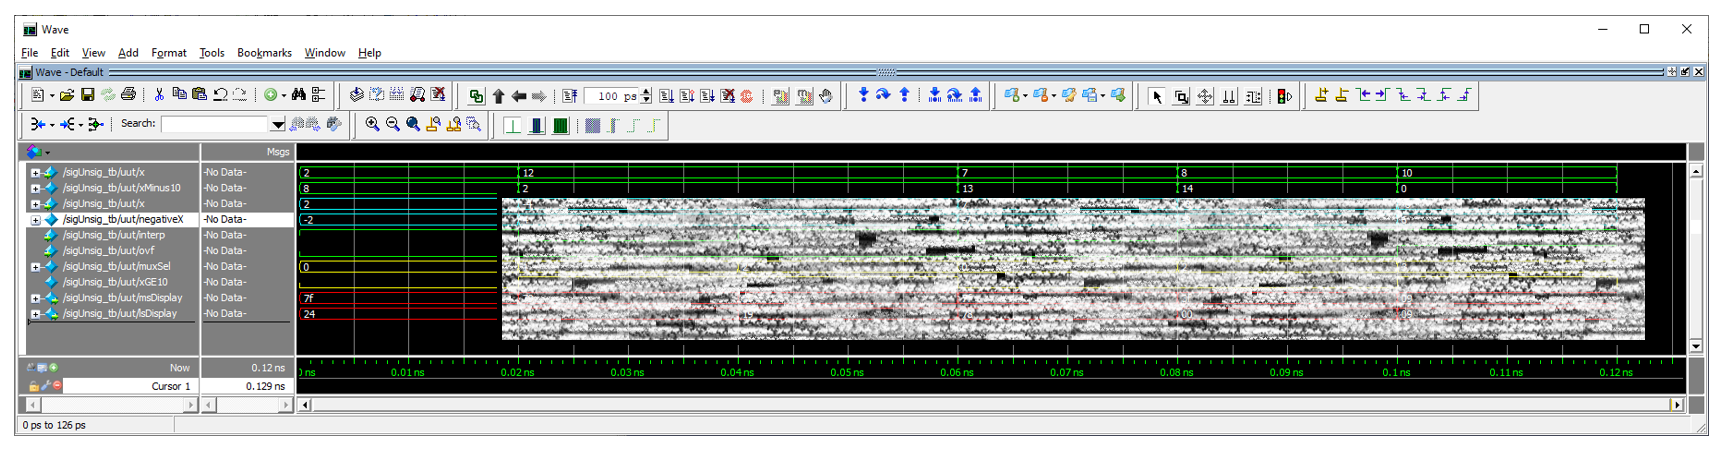
\includegraphics{ image7.png}

\subsubsection{Pin-Assignment}

Complete the pin assignment in table~\ref{table:calcPinAssignment}.

